%
% fig/argument.tex -- Geometrische Anschauung des Argumentprinzips
%
\begin{figure}
\centering
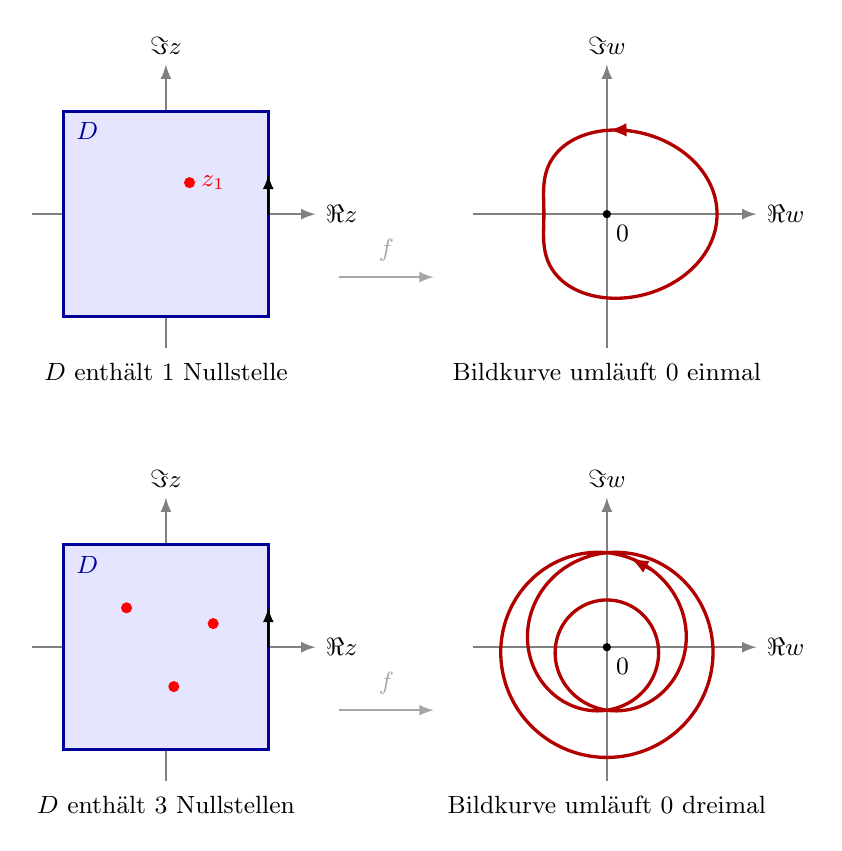
\begin{tikzpicture}[>=latex,thick,scale=1.0]
%
% Zwei Paare: Urbildebene (links) und Bildebene (rechts)
% Fall 1: D enthält 1 Nullstelle -> Bildkurve umläuft 0 einmal
% Fall 2: D enthält 3 Nullstellen -> Bildkurve umläuft 0 dreimal
%
% --- Fall 1: 1 Nullstelle ---
\begin{scope}[yshift=0cm]
  % Urbildebene
  \begin{scope}[xshift=0cm]
    % Achsen
    \draw[->,gray] (-1.7,0) -- (1.9,0) node[right,black]{\small$\Re z$};
    \draw[->,gray] (0,-1.7) -- (0,1.9) node[above,black]{\small$\Im z$};
    % Gebiet D (Quadrat)
    \draw[blue!60!black,line width=1pt,fill=blue!10] (-1.3,-1.3) rectangle (1.3,1.3);
    \node[blue!60!black] at (-1.0,1.05) {\small $D$};
    % Eine Nullstelle
    \fill[red] (0.3,0.4) circle (2pt);
    \node[red] at (0.6,0.4) {\small $z_1$};
    % Pfeil entlang Rand
    \draw[->,thick] (1.3,0) -- (1.3,0.5);
    \node at (0,-2.0) {\small $D$ enthält $1$ Nullstelle};
  \end{scope}
  % Pfeil zwischen Urbild und Bild (etwas tiefer, Label leicht nach oben geschoben)
  \draw[->,thick,gray!70] (2.2,-0.8) -- (3.4,-0.8) node[midway,above,yshift=2pt]{\small $f$};
  % Bildebene: Schleife einmal um 0
  \begin{scope}[xshift=5.6cm]
    \draw[->,gray] (-1.7,0) -- (1.9,0) node[right,black]{\small$\Re w$};
    \draw[->,gray] (0,-1.7) -- (0,1.9) node[above,black]{\small$\Im w$};
    \fill[black] (0,0) circle (1.5pt);
    \node at (0.2,-0.25) {\small $0$};
    % Schleife einmal um 0 (Ellipse, verzerrt)
    \draw[red!70!black,line width=1.2pt,smooth,samples=80,domain=0:360]
      plot ({1.1*cos(\x)+0.3*cos(2*\x)},{1.0*sin(\x)+0.2*sin(2*\x)});
    % Pfeil-Richtung auf Kurve
    \draw[->,red!70!black,line width=1.2pt]
      ({1.1*cos(70)+0.3*cos(140)},{1.0*sin(70)+0.2*sin(140)})
      -- ({1.1*cos(75)+0.3*cos(150)},{1.0*sin(75)+0.2*sin(150)});
    \node at (0,-2.0) {\small Bildkurve umläuft $0$ einmal};
  \end{scope}
\end{scope}
%
% --- Fall 2: 3 Nullstellen ---
\begin{scope}[yshift=-5.5cm]
  \begin{scope}[xshift=0cm]
    \draw[->,gray] (-1.7,0) -- (1.9,0) node[right,black]{\small$\Re z$};
    \draw[->,gray] (0,-1.7) -- (0,1.9) node[above,black]{\small$\Im z$};
    \draw[blue!60!black,line width=1pt,fill=blue!10] (-1.3,-1.3) rectangle (1.3,1.3);
    \node[blue!60!black] at (-1.0,1.05) {\small $D$};
    \fill[red] (-0.5,0.5) circle (2pt);
    \fill[red] (0.6,0.3) circle (2pt);
    \fill[red] (0.1,-0.5) circle (2pt);
    \draw[->,thick] (1.3,0) -- (1.3,0.5);
    \node at (0,-2.0) {\small $D$ enthält $3$ Nullstellen};
  \end{scope}
  \draw[->,thick,gray!70] (2.2,-0.8) -- (3.4,-0.8) node[midway,above,yshift=2pt]{\small $f$};
  \begin{scope}[xshift=5.6cm]
    \draw[->,gray] (-1.7,0) -- (1.9,0) node[right,black]{\small$\Re w$};
    \draw[->,gray] (0,-1.7) -- (0,1.9) node[above,black]{\small$\Im w$};
    \fill[black] (0,0) circle (1.5pt);
    \node at (0.2,-0.25) {\small $0$};
    % Dreifach um 0: r(t) mit Variation, Winkel 3t
    \draw[red!70!black,line width=1.2pt,smooth,samples=200,domain=0:360]
      plot ({(1.0+0.4*sin(\x))*cos(3*\x)},{(1.0+0.4*sin(\x))*sin(3*\x)});
    % Pfeil-Richtung
    \draw[->,red!70!black,line width=1.2pt]
      ({(1.0+0.4*sin(20))*cos(60)},{(1.0+0.4*sin(20))*sin(60)})
      -- ({(1.0+0.4*sin(25))*cos(75)},{(1.0+0.4*sin(25))*sin(75)});
    \node at (0,-2.0) {\small Bildkurve umläuft $0$ dreimal};
  \end{scope}
\end{scope}
\end{tikzpicture}
\caption{Geometrische Bedeutung des Wegintegrals: läuft $z$ einmal um den Rand
$\partial D$ eines Gebiets, so umrundet der Bildpunkt $f(z)$ den Ursprung in der
Bildebene genau so oft, wie $f$ Nullstellen in $D$ besitzt. Oben: $D$ enthält
eine Nullstelle, die Bildkurve $f(\partial D)$ macht eine Drehung um $0$.
Unten: $D$ enthält drei Nullstellen, die Bildkurve umläuft den Ursprung dreimal.
\label{weyl:fig:argument}}
\end{figure}
